\chapter{Experimenteller Aufbau}
\begin{figure}
    \centering
    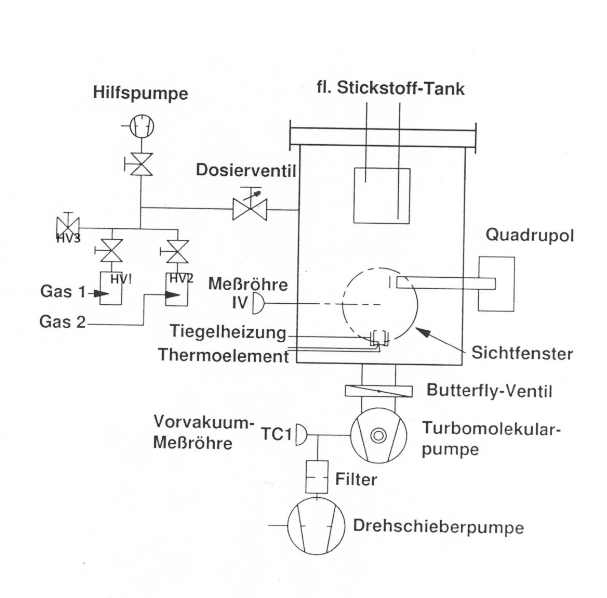
\includegraphics[width=130mm,scale=0.8]{Massenspektrometer/include/Massenspektrometer_Aufbau.png}
    \caption{Aufbau des Experiments \cite{VorbereitungsMappe}(bearbeitet)}
    \label{fig:aufbau}
\end{figure}
Das Experiment ist entsprechend  Abbildung \ref{fig:aufbau} aufgebaut. Durch die Handventile HV1-3 kann Argon, Propan oder Raumluft ins System gebracht werden. Das System kann unter Verwendung der Hilfspumpe gespült werden, indem mehrmals das gewünschte Gas eingelassen und mit der Hilfpumpe abgepumpt wird. Dabei sollte das Dosierventil beinahe geschlossen sein, damit die Vakuumkammer keine plötzliche Druckänderung erfährt, was das Massenspektrometer und die Turbomolekularpumpe beschädigen könnte. Über das Dosierventil kann der Gasfluss in die Vakuumkammer sehr präzise reguliert werden. Die Vakuumkammer wird mit einer Drehschieberpumpe und einer Turbomolekularpumpe abgepumpt. Die Turbomolekularpumpe ist sehr effizient darin ein Hochvakuum zu erzeugen, benötigt jedoch bevor sie eingesetzt werden kann ein Vorvakuum (Feinvakuum), welches von der Drehschieberpumpe erzeugt wird. In der Vakuumkammer befindet sich eine Tiegelheizung mit Thermoelement, wodurch die Temperatur in der Kammer reguliert und abgelesen werden kann. Angeschlossen an die Vakuumkammer ist das Ionisationsmanometer, welches verwendet werden kann um den Druck zu messen und das Quadrupolmassenspektrometer, dessen Funktion bereits in Kapitel \ref{chapter:QMS} erläutert wurde.